% ShelfSense weekly report 4 (replaces the Report 4 part of reports_3_4.tex, which followed an
% older draft of Report 3). Paste into the Overleaf main file in place of the empty
% "\section{Weekly Report 4}" heading. Upload the files in figures/ to the Overleaf project and add the
% entries in new_refs.bib to ref.bib. Needs \usepackage{xcolor} and
% \newcommand{\TODO}[1]{\textcolor{red}{[#1]}} in the preamble. Lines marked \TODO{...} need a team member.

\section{Weekly Report 4}

\subsection{Follow-up from last week}
Status of the targets set in Weekly Report 3:
\begin{enumerate}
  \item \textbf{SKU-110K training subset in YOLO format --- Done (larger).} We prepared 2{,}000
  training and 500 validation images instead of 1{,}500 and 300, and later a 4{,}000-image training
  set (Section~\ref{sec:r4-det}).
  \item \textbf{Fine-tune YOLOv8n and report mAP --- Done.} mAP@0.5 \TODO{4k: 0.913} and
  mAP@0.5:0.95 \TODO{4k: 0.564} on 500 held-out SKU-110K images. Training ran on a team laptop with a
  GTX~1650 GPU instead of Kaggle: it has no weekly time limit and no upload of the dataset is needed.
  \item \textbf{Detector vs.\ VLM counting on 20 SKU-110K images --- Done.} See
  Section~\ref{sec:r4-count}.
  \item \textbf{Empty-gap labels from the synthetic generator --- Changed.} Empty gaps on real
  shelves look very different from the flat gaps of generated images. We instead label
  \emph{empty\_gap} boxes directly on our own video frames; 222 frames are pre-labelled and ready for
  correction (Section~\ref{sec:r4-det}).
  \item \textbf{ONNX export and CPU timing --- Done.} See Section~\ref{sec:r4-cpu}.
\end{enumerate}

\textbf{Corrections to Report 3.} The results section of Report~3 was submitted before the Kaggle
run had finished and still showed a placeholder. The baseline was run, but on real footage instead of
the synthetic shelves: we obtained phone videos of branded beverage fridges in Bangladeshi shops and
used them instead of generated images. Section~\ref{sec:r4-baseline} gives the actual baseline
results. Two further changes since Report~2 are also described there: the blur metric of the keyframe
extractor, and the model precision (float16, not float32).
\TODO{Team: if the synthetic set (make\_eval\_set.py) or simulator code exists, add it to the GitHub
repo; otherwise keep this paragraph as it is.}

\subsection{Work narrative of the current week}
This week covered Sprint 4: a product detector that counts what the VLM cannot. We also completed
the baseline promised in Report~3 and recorded our first larger real dataset.

\subsubsection{Refined problem: verifiable audits}
Our team's knowledge of Bangladeshi retail sharpened the problem. Brand companies (for example
Coca-Cola, Pepsi/Transcom and Akij) give shops branded fridges on condition that only their
products are stored inside, and pay shops for prime placement. A first real client, NutriCoco
(Coco Fresh coconut pudding), pays shops in Mirpur about 135\,Tk per day to keep its cups at the
front of the shop fridge and today has no way to check this. Field auditors are sometimes bribed by
shopkeepers and report false compliance. ShelfSense must therefore replace the auditor's word with
evidence: every finding points to a keyframe, a timestamp and later a bounding box that a person can
check. Two design rules follow:
\begin{itemize}
  \item \textbf{New key KPIs:} \emph{cooler purity} (only the owner's brands in a branded fridge)
  and \emph{paid placement} (the agreed brand on the agreed shelf or at the front).
  \item \textbf{Precision over recall for violations:} a false ``competitor in your fridge''
  accuses an honest shopkeeper, so invented brands are unacceptable.
\end{itemize}

\subsubsection{Baseline VLM on real fridge videos (Report 3 results)}\label{sec:r4-baseline}
\textbf{Data and blur metric.} Our first real footage was three short WhatsApp clips of branded
fridges (576$\times$1024 portrait, 2.3\,s, 6.4\,s and 2.4\,s). On these the adaptive Laplacian
threshold from Report~2 failed: the Laplacian variance depends on scene content, so sharp close-ups
scored 49 while motion-blurred frames scored 147, and no threshold separated them. We replaced it
with the no-reference \emph{blur effect} of Crete et al.\ \cite{crete2007blur}, which compares a
frame with a re-blurred copy of itself and gives 0 for sharp and 1 for fully blurred images. Real
frames scored 0.24--0.39 and artificially blurred copies 0.56--0.72, so frames above 0.5 are
dropped. The Laplacian score is still logged for comparison.

\textbf{Setup.} Qwen2-VL-2B-Instruct \cite{wang2024qwen2vl}, zero-shot, float16 on a Kaggle T4
(it ran without overflow), greedy decoding, at most 256 new tokens. Five prompts, each with a JSON
answer: fridge brand, product brands, counts per brand, empty space and price tags. Every question
is asked in \emph{image mode} (each keyframe separately, answers combined per video) and
\emph{video mode} (up to 8 keyframes given to the model as one video). Version~2 of the prompts
targeted each version~1 failure: look only behind the glass door, list each brand once, do not
guess common brands, ignore shop signs, and give explicit empty answers. Model, image size and
generation settings stayed fixed, so the versions differ only in the prompts.
Table~\ref{tab:r4-baseline} gives the results and Table~\ref{tab:r4-failures} the failure cases.
The ground truth for the three videos was labelled by hand; the brands in the third video (red cans
that may be Mojo rather than Coca-Cola) are still being double-checked, so small changes in the
brand scores are possible.

\begin{table}[!t]
\centering
\caption{Baseline Qwen2-VL-2B on three fridge videos (image / video mode).}
\label{tab:r4-baseline}
\begin{tabular}{lcc}
\hline
Metric & Prompt v1 & Prompt v2 \\
\hline
Unparseable answers & 22 / 2 & 8 / 0 \\
Mean time per answer (s) & 3.6 & 2.9 \\
Fridge brand accuracy & 0.67 / 0.33 & 0.67 / 0.67 \\
Brand precision & 0.27 / 0.30 & 0.13 / 0.25 \\
Brand recall & 1.00 / 0.50 & 1.00 / 1.00 \\
Empty space accuracy & 0.33 / 0.67 & 0.67 / 0.67 \\
Price tag accuracy & 0 / 0 & 0.33 / 0 \\
\hline
\end{tabular}
\end{table}

\begin{table}[!t]
\centering
\caption{Typical failure cases of the zero-shot VLM.}
\label{tab:r4-failures}
\begin{tabular}{p{0.28\linewidth}p{0.62\linewidth}}
\hline
Failure & Example \\
\hline
Invented brands & Pepsi, 7up and Dr Pepper listed in a Coca-Cola fridge \\
No real counting & Every count 10 (or 1) in v1; 10/10/10 or 0/0/0 in v2 \\
Invented price tags & Sequences such as 1, 2, 3 or TK 10, TK 15; the \texttt{<price>} placeholder copied \\
Repetition loops & The same brand repeated until the token limit \\
Wrong text read & Shop sign or ``property of'' text given as the fridge brand; ``nojo'' for Mojo \\
Limits become targets & ``At most 8 brands'' $\rightarrow$ exactly 8 brands; ``at most 5 prices'' $\rightarrow$ 5 invented prices \\
\hline
\end{tabular}
\end{table}

Better prompts fixed the \emph{format} problems: unparseable answers fell from 24 to 8, repetition
loops stopped and answers became faster. They did not fix \emph{perception}: brand precision got
worse (0.27 $\rightarrow$ 0.13 in image mode) because the model listed brands that are commonly sold
rather than brands it could see, and counts were never real. With three videos these numbers show
failure patterns, not significant differences. We stopped prompt tuning: the detector must count,
and the VLM should be asked about one product at a time (Section~\ref{sec:r4-crops}).

\subsubsection{New footage and dataset statistics}\label{sec:r4-data}
We received 119 video files from one Bangladeshi supermarket. SHA-256 hashes showed that 4 were
byte-identical copies, and 4 were wide stock clips of whole aisles that we excluded, leaving 111 own
recordings (576$\times$1024, median 11\,s, about 21 minutes). They show open shelves of personal
care, biscuits and snacks, noodles, tea and coffee, juices, soft drinks, cereal, milk, rice and
lentils and oil, with Taka price tags visible. Neighbouring clips film the same shelf, so we split
the videos into training and test sets by blocks of consecutive videos; frames of one shelf never
appear in both sets. Table~\ref{tab:r4-data} gives the extraction statistics at 4\,fps.

\begin{table}[!t]
\centering
\caption{Keyframe extraction on the 111 supermarket videos (4\,fps).}
\label{tab:r4-data}
\begin{tabular}{lrrrrrr}
\hline
Split & Videos & Duration (s) & Sampled & Kept & Blurry & Duplicate \\
\hline
Train & 82 & 934 & 3{,}771 & 3{,}420 & 54 & 297 \\
Test & 29 & 322 & 1{,}298 & 1{,}071 & 115 & 112 \\
\hline
\end{tabular}
\end{table}

These videos contain the first real motion blur we have seen. The blur effect ranked frames
correctly (sharp frames 0.25--0.35, smeared frames 0.58--0.62, Fig.~\ref{fig:r4-blur}), but frames
near the 0.5 threshold can go either way, so we kept 0.5. For annotation, a script picks the
sharpest frame in each half of every video: 164 training and 58 test keyframes.

\begin{figure}[!t]
\centering
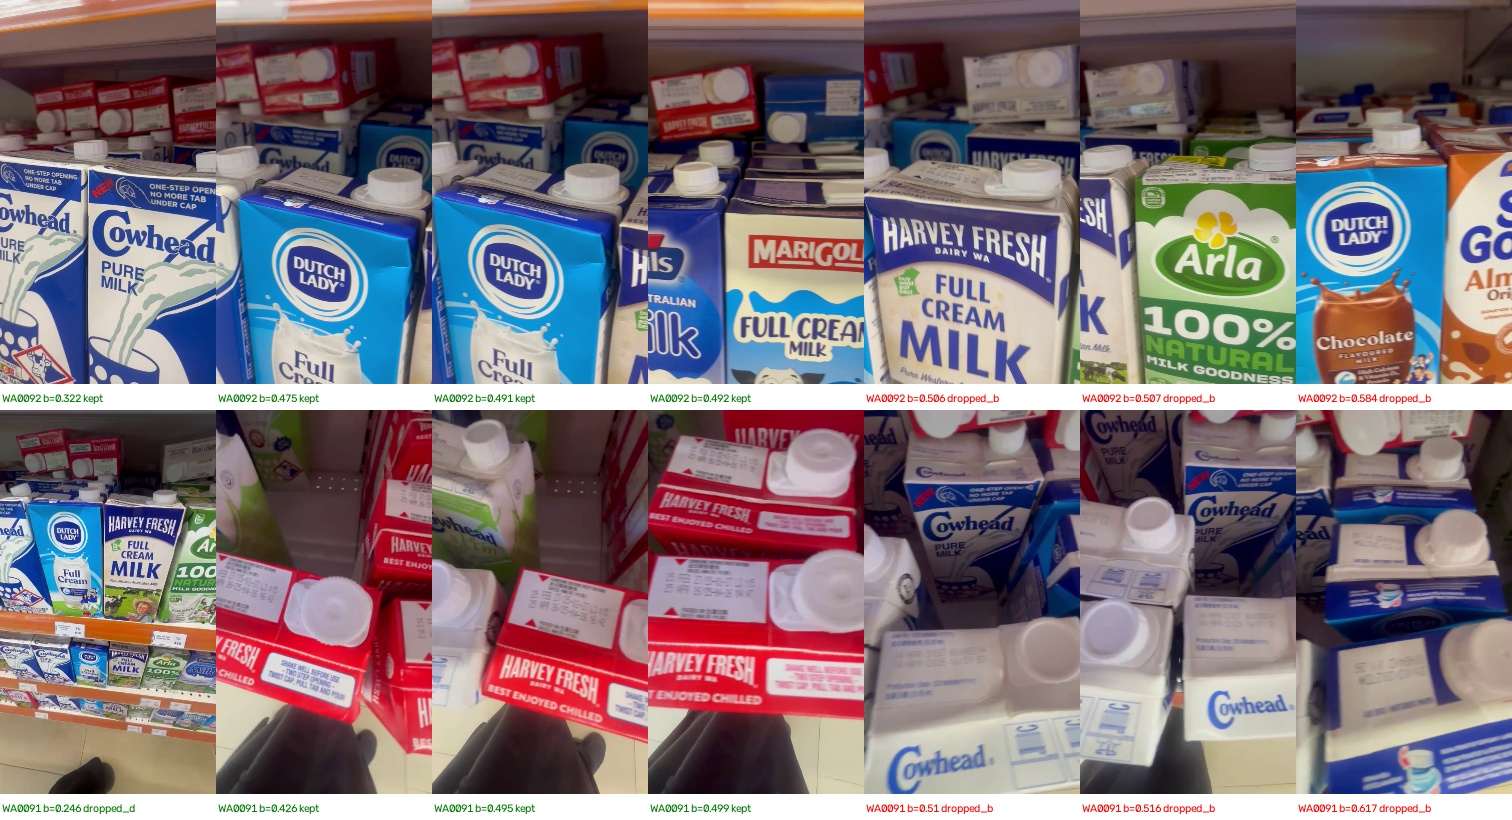
\includegraphics[width=\linewidth]{figures/blur_check.jpg}
\caption{Real motion blur in two milk-carton videos. Green: kept, red: dropped by the blur filter
(blur effect $b$ above 0.5).}
\label{fig:r4-blur}
\end{figure}

\subsubsection{Product detector}\label{sec:r4-det}
We trained YOLOv8n \cite{jocher2023yolov8,redmon2016yolo} with one class, \emph{product} (no
brands), on a random subset of SKU-110K \cite{goldman2019sku110k}. SKU-110K photos are up to about
4{,}000 pixels wide, so we shrank them once to 1{,}280 pixels to keep data loading fast. The first
model was trained on 2{,}000 images for 30 epochs at 1{,}024 pixels (163.5 minutes on a GTX~1650
with 4\,GB). Its mAP was still rising at the last epoch, so we continued training it for
\TODO{20} more epochs on 4{,}000 images (a superset of the first 2{,}000, same 500 validation
images, \TODO{minutes}). Table~\ref{tab:r4-det} shows the results and two settings that matter for
dense shelves.

\begin{table}[!t]
\centering
\caption{YOLOv8n on the same 500 SKU-110K validation images.}
\label{tab:r4-det}
\begin{tabular}{lcccc}
\hline
Model and setting & mAP50 & mAP50-95 & Precision & Recall \\
\hline
2k images, 1{,}024\,px, max.\ 1{,}000 boxes & 0.913 & 0.564 & 0.897 & 0.844 \\
2k images, 1{,}024\,px, max.\ 299 boxes & 0.889 & 0.549 & 0.897 & 0.833 \\
2k images, 640\,px, max.\ 1{,}000 boxes & 0.866 & 0.510 & 0.875 & 0.792 \\
\TODO{4k images, 1{,}024\,px, max.\ 1{,}000 boxes} & \TODO{} & \TODO{} & \TODO{} & \TODO{} \\
\hline
\end{tabular}
\end{table}

\begin{figure}[!t]
\centering
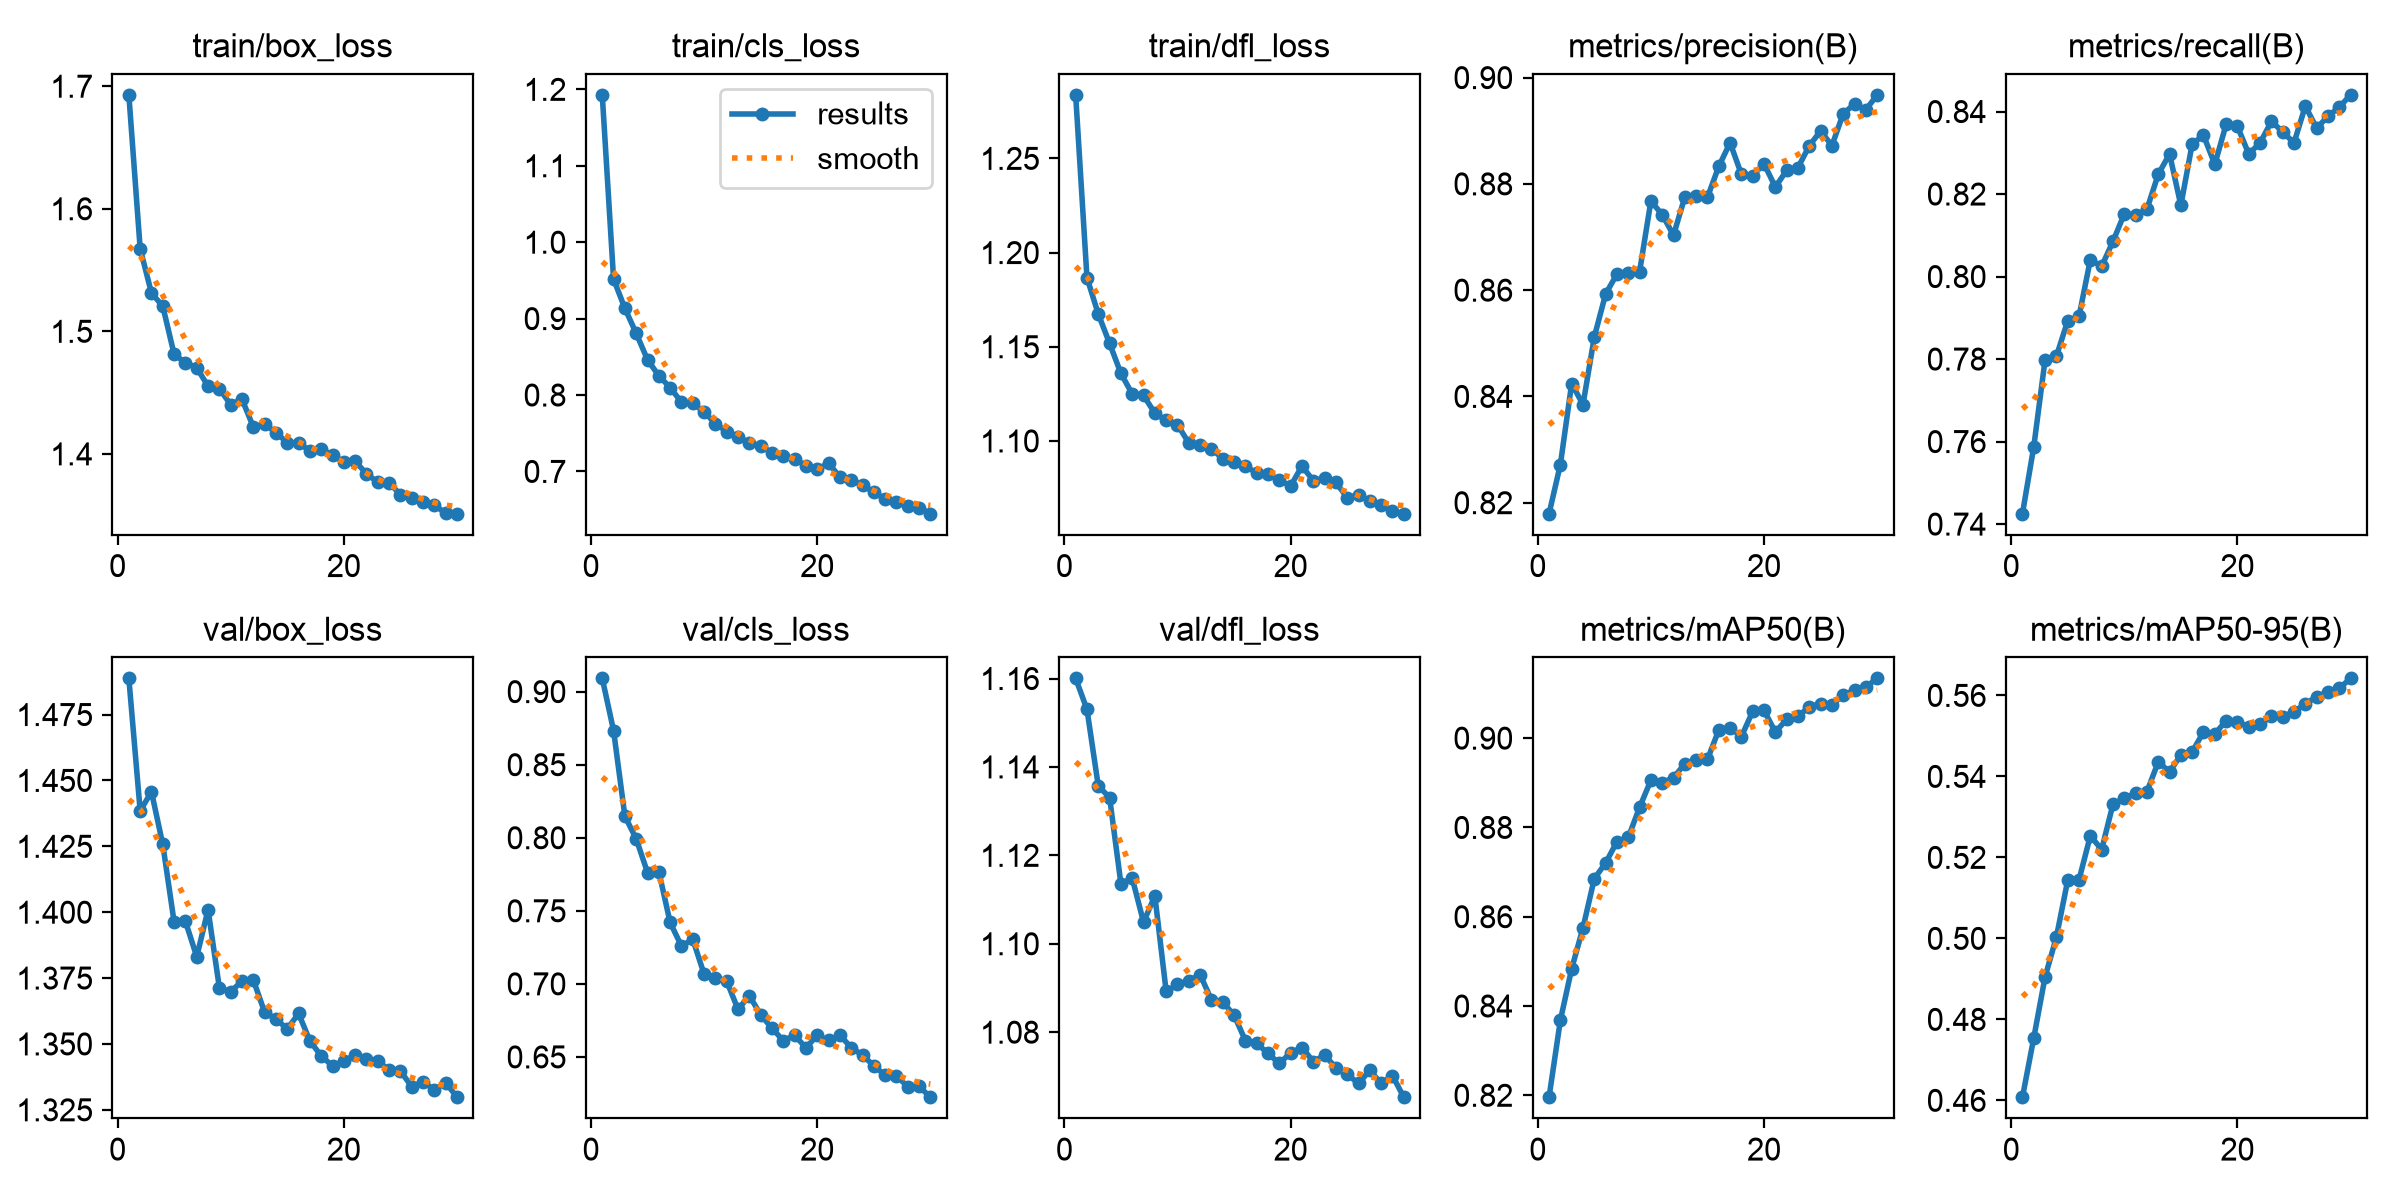
\includegraphics[width=\linewidth]{figures/sku110k_training_curves.png}
\caption{Training curves of the first model. Losses fall on both training and validation data, and
mAP is still rising at epoch 30.}
\label{fig:r4-curves}
\end{figure}

\begin{itemize}
  \item \textbf{Detection limit.} One validation image holds 718 products and 11 of 500 hold more
  than 300, so Ultralytics' default limit of 300 boxes per image costs 2.4 mAP50 points. We use
  1{,}000.
  \item \textbf{Image size.} Products are small, so the default 640\,px input costs 4.7 mAP50
  points against 1{,}024\,px.
  \item \textbf{More data.} \TODO{effect of 4k images}
  \item \textbf{On our footage.} The detector found 151{,}279 products on our 4{,}558 keyframes,
  a median of 29 per frame. It boxes nearly every item on packed shelves seen from a normal
  distance, but misses large products close to the camera (Fig.~\ref{fig:r4-detect}). Milk-carton
  close-ups get a median of 6 boxes per frame, against 53 for canned food, because SKU-110K
  products are small in the image.
  \item \textbf{mAP on our own frames} needs corrected labels and is carried over. The detector's
  boxes on the 222 annotation frames (median 30 per frame) are ready to be corrected in Roboflow,
  together with hand-drawn \emph{empty\_gap} boxes; correcting is much faster than drawing every box.
\end{itemize}

\begin{figure}[!t]
\centering
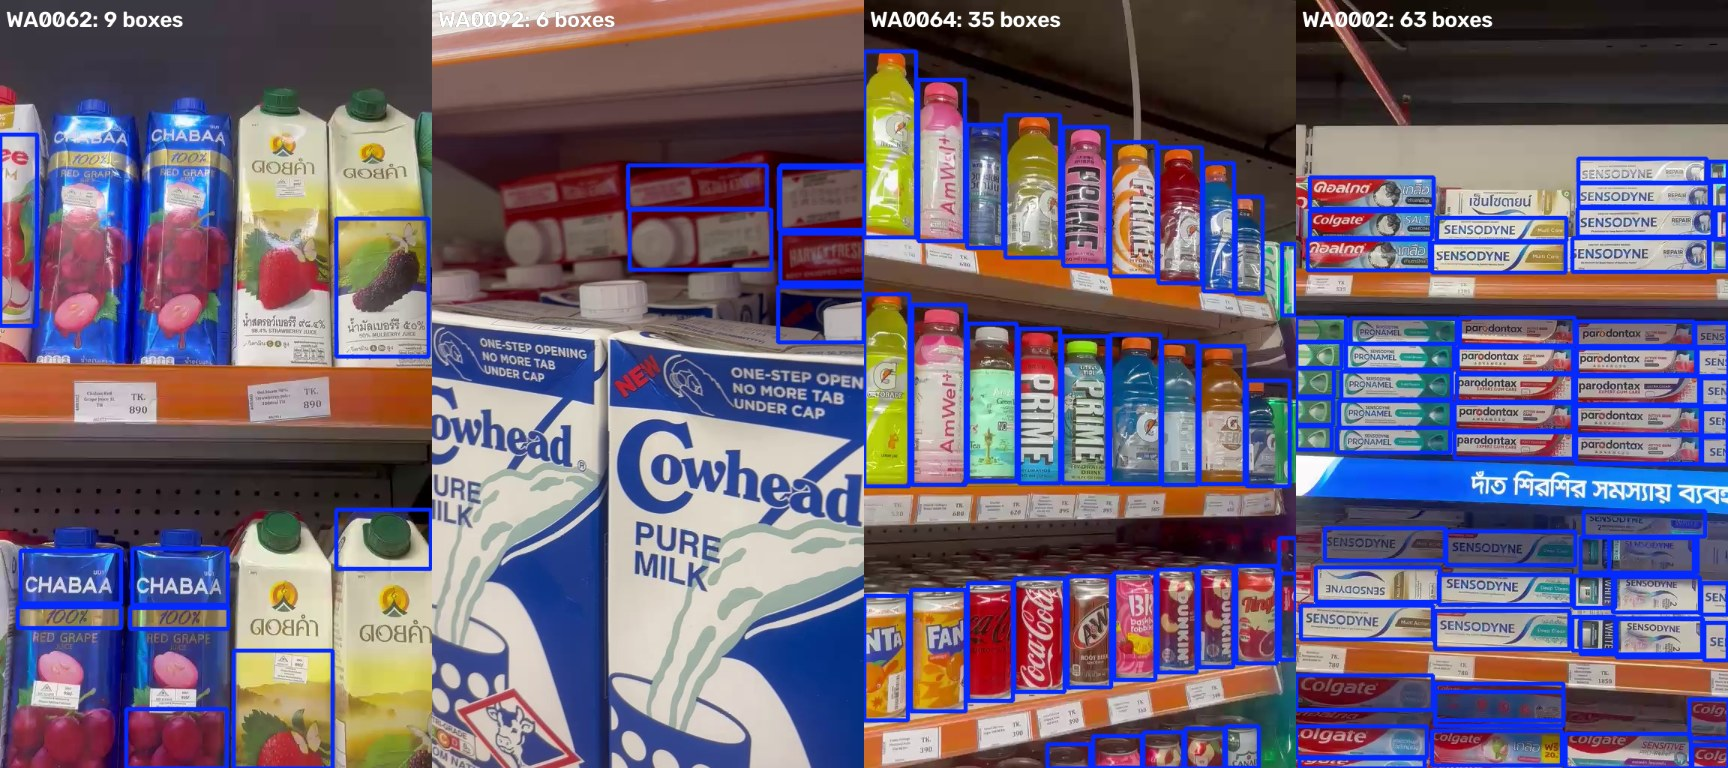
\includegraphics[width=\linewidth]{figures/detector_good_and_bad.jpg}
\caption{Detector output on our test videos. Left two: large close-up cartons are missed or split.
Right two: packed shelves at normal distance, where nearly every product is found.}
\label{fig:r4-detect}
\end{figure}

\subsubsection{Counting: detector vs.\ VLM}\label{sec:r4-count}
We took 20 random images from the SKU-110K \emph{test} split, which was used for neither training
nor validation; the true count of an image is its number of annotated boxes (108--178, mean 131.6).
The VLM was asked the counting prompt of Report~3 (\emph{``Count every individual product facing
\ldots''}, JSON answer). The detector counts its boxes above a confidence threshold. The default of
0.25 overcounts, so we chose the threshold that counts best on the 500 validation images (0.35,
validation MAE 19.7 $\rightarrow$ 16.0) and then applied it to the test images unchanged.
Table~\ref{tab:r4-count} gives the result.

\begin{table}[!t]
\centering
\caption{Product counting on 20 SKU-110K test images (true count 108--178).}
\label{tab:r4-count}
\begin{tabular}{lcccc}
\hline
Method & MAE & MAPE & Within 10\% & Undercounted \\
\hline
Qwen2-VL-2B (zero-shot) & \TODO{} & \TODO{} & \TODO{} & \TODO{} \\
YOLOv8n, conf 0.25 (default) & 21.4 & 15.7\% & 50\% & 20\% \\
YOLOv8n, conf 0.35 (tuned on val) & 15.8 & 11.6\% & 70\% & 45\% \\
\TODO{YOLOv8n 4k} & \TODO{} & \TODO{} & \TODO{} & \TODO{} \\
\hline
\end{tabular}
\end{table}

\TODO{interpretation after VLM run}

\subsubsection{CPU inference}\label{sec:r4-cpu}
The team laptops have no NVIDIA GPU, so the detector must run on the CPU. We exported it to ONNX
with a fixed 1{,}024$\times$576 input that matches our portrait frames (a 1{,}024$\times$1{,}024
square would be 44\% padding) and timed it on 30 of our test keyframes, after three warm-up frames
(Table~\ref{tab:r4-cpu}). The ONNX model gave exactly the same box counts as PyTorch, but on this
CPU it was slower, so we keep PyTorch. At about 0.1\,s per keyframe, a 30-second video sampled at
1\,fps is processed in about 3\,s, so the detector is not the bottleneck of the pipeline; the VLM
is (Section~\ref{sec:r4-crops}).

\begin{table}[!t]
\centering
\caption{Detector inference time on the CPU (Intel Core i7-8565U, 30 frames of 576$\times$1{,}024).}
\label{tab:r4-cpu}
\begin{tabular}{lccc}
\hline
Runtime & Median (ms/frame) & Frames per second & Model size \\
\hline
PyTorch (CPU) & 106 & 9.5 & 6.2\,MB \\
ONNX Runtime (CPU) & 142 & 7.1 & 12.8\,MB \\
\hline
\end{tabular}
\end{table}

\subsubsection{Brand reading on product crops}\label{sec:r4-crops}
To test whether the VLM reads brands better one product at a time, we took the 12 annotation frames
of the six drinks-shelf test videos, cut 120 random detector crops, and asked the same Qwen2-VL-2B
model (float16, zero-shot) ``which brand is this?'' for each crop and ``list the brands'' for each
whole frame. Answers were matched to a catalogue of the 24 expected brands, as an audit for a brand
company would; the catalogue was built from our labels, so this is an upper bound.
Table~\ref{tab:r4-crops} shows the result and Fig.~\ref{fig:r4-crops} gives examples.

\begin{table}[!t]
\centering
\caption{Brand reading on 12 drinks-shelf frames: whole frame vs.\ detector crops (Qwen2-VL-2B).}
\label{tab:r4-crops}
\begin{tabular}{lccc}
\hline
Method & Usable answers & Brand precision & Brand recall \\
\hline
Whole frame & 6 of 12 & 1.00 (6 frames) & 0.30 \\
Detector crops & 12 of 12 & 0.94 & \textbf{0.63} \\
\hline
\end{tabular}
\end{table}

\begin{figure}[!t]
\centering
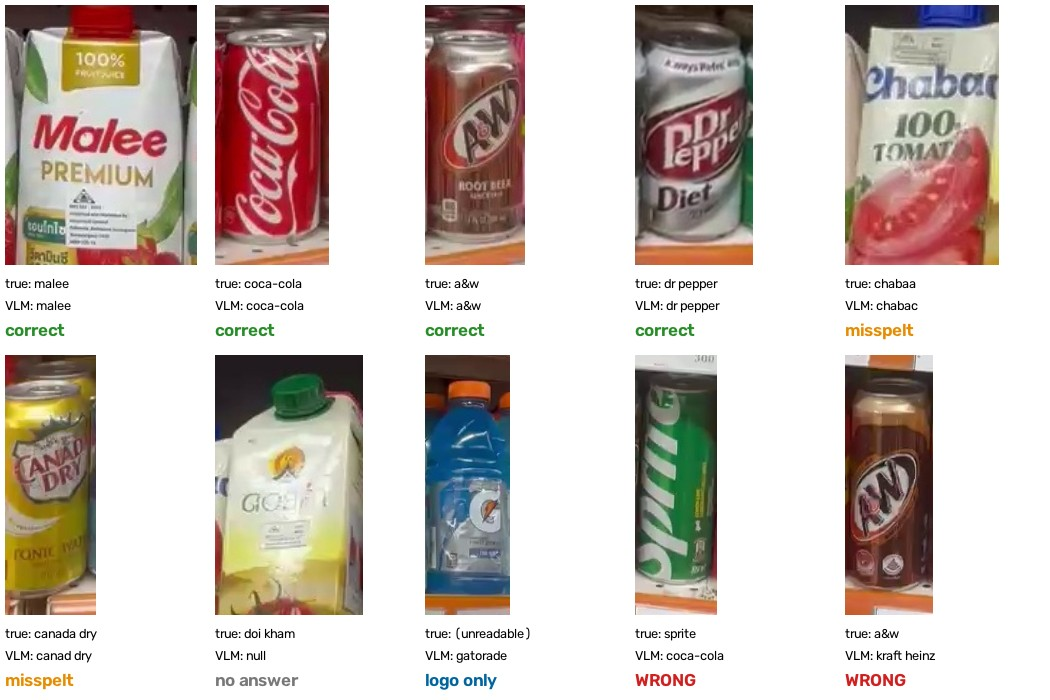
\includegraphics[width=\linewidth]{figures/crop_brand_examples.jpg}
\caption{Examples of single-product crops with the true brand and the VLM answer.}
\label{fig:r4-crops}
\end{figure}

\begin{itemize}
  \item Crops \textbf{doubled the brand recall} (0.30 $\rightarrow$ 0.63) at high precision. Six of
  the twelve whole-frame answers repeated words until the token limit and gave no usable list,
  the same loop seen in the baseline.
  \item Per crop, 48 of 67 readable crops were named correctly (72\%; 67\% before catalogue
  matching). Many raw answers are near-misses (``chabac'', ``canad dry'') that the catalogue fixes.
  \item Wrong brands are rare but biased: 2 of 120 crops were named ``Coca-Cola'' (for Canada Dry
  and Sprite), the same pull towards famous brands as in the baseline. A human must still check the
  evidence crop before a violation is reported.
  \item No answer was given for 11 readable crops, mostly brands written in Thai or Bengali script.
  \item Speed: 21\,s per crop on the 4\,GB GPU, because the model does not fit and is partly kept in
  CPU memory. A frame with 30 products would take 10 minutes; Sprint~5 must ask only about the
  products that matter for the audit (for example one crop per position in the paid zone).
\end{itemize}
The crop and frame labels were drafted for this test and still need a second check by the team.

\subsubsection{Challenges faced}
\begin{itemize}
  \item \textbf{The new footage shows open shelves, not branded fridges.} It is ideal for product
  detection, share of shelf and price tags, but cooler purity still needs fridge recordings.
  \item \textbf{4\,GB of GPU memory.} A batch of 8 images at 1{,}024\,px needs 7.5\,GB and a batch of
  4 still overflowed on dense images, slowing training 2.7 times; we trained with batches of 2.
  Each data-loading worker also loaded its own copy of PyTorch, which exhausted Windows memory,
  so we used one worker.
  \item \textbf{A hidden default.} Ultralytics silently raises the 300-box limit during validation,
  which at first made our 300 vs.\ 1{,}000 comparison meaningless; we re-measured with 299.
  \item \textbf{ONNX was not faster.} Exporting to ONNX is often recommended for CPU speed, but on
  our CPU PyTorch was 25\% faster, so we measured instead of assuming.
  \item \textbf{Licence.} SKU-110K may be used for academic, non-commercial work only and must not
  be redistributed, so its photos stay on our machine.
\end{itemize}

\subsubsection{Progress made}
Sprint~4 is mostly complete: the detector is trained and evaluated on SKU-110K, counts far better
than the VLM, runs on a laptop CPU, and the crop test supports the hybrid design. The Report~3
baseline is now reported. The remaining Sprint~4 item is mAP on our own frames, which needs the
corrected labels.

\subsection{Target for next weekly update}
\begin{enumerate}
  \item Correct the pre-labels on the 222 keyframes in Roboflow, including empty-gap boxes; two
  members check every test frame.
  \item Fine-tune the detector on our 164 training frames and report mAP and counting error on our
  58 test frames, before and after fine-tuning.
  \item Verify the crop brand labels and the baseline ground truth.
  \item Record shop fridges (15--30\,s each), including NutriCoco's paid front zone and fridges with
  competitor products, to test paid placement and cooler purity.
  \item Start Sprint~5: connect extraction, detection and the VLM into one pipeline that writes a
  JSON audit report with evidence (keyframe, timestamp, box) for every finding.
\end{enumerate}

\subsection{Individual contribution}
\begin{table}[!h]
\centering
\caption{Contribution summary.}
\begin{tabular}{lcc}
\hline
Task List & Member Assigned & Comments \\
\hline
Baseline VLM run and failure analysis (Report 3 results) & \TODO{member} & Prompts v1, v2 \\
Supermarket video recording & \TODO{member} & 115 videos \\
Video inventory, split and extraction & \TODO{member} & 4{,}558 keyframes \\
SKU-110K detector training and evaluation & \TODO{member} & 2k and 4k images \\
Counting comparison and CPU timing & \TODO{member} & Detector vs.\ VLM, ONNX \\
Pre-labels and annotation frame selection & \TODO{member} & 222 frames \\
VLM crop test and brand labels & \TODO{member} & Recall 0.30 $\rightarrow$ 0.63 \\
\hline
\end{tabular}
\end{table}
